\documentclass[a4paper,12pt]{extarticle}
\usepackage[table,xcdraw]{xcolor}
\usepackage{pgfplots}
\usepackage[unicode, pdftex]{hyperref}
\usepackage[T2A]{fontenc}
\usepackage[utf8]{inputenc}
\usepackage[english,russian]{babel}
\usepackage{amsmath,amsfonts,amsthm, mathtools}
\usepackage{amssymb}
\usepackage{graphicx}
\graphicspath{{images/}}
\usepackage{wrapfig}
\usepackage{floatrow}
\usepackage{setspace}
\usepackage[headings]{fancyhdr}
\usepackage[margin=10pt,font={small,stretch=0,9},labelfont=bf,labelsep=period,
justification=centerlast]{caption}
\usepackage{array,tabularx,tabulary,booktabs}
\RequirePackage{multirow}
\RequirePackage{multicol}
\RequirePackage{longtable}
\usepackage{indentfirst}
\usepackage{hyperref}
\usepackage{icomma}
\newcommand*{\hm}[1]{#1\nobreak\discretionary{}
	{\hbox{$\mathsurround=0pt #1$}}{}}
\usepackage{soulutf8} 
\usepackage{etoolbox} 
\usepackage{geometry}
\geometry{top=20mm}
\geometry{bottom=20mm}
\geometry{left=20mm}
\geometry{right=20mm}
\DeclareMathOperator{\sgn}{\mathop{sgn}}
\usepackage[OT1]{fontenc}
\usepackage{amsmath}
\usepackage{amsfonts}
\usepackage{amssymb}
\usepackage{wasysym}
\usepackage{wrapfig}
\usepackage{physics}
\usepackage[normalem]{ulem}
\graphicspath{{pictures/}}
\DeclareGraphicsExtensions{.png,.jpg,.jpeg}
\usepackage{indentfirst}
\usepackage[T2A]{fontenc}
\usepackage{subfigure}
\usepackage{fancyhdr}
\usepackage{caption}

\usepackage{tabularx}
\usepackage{floatrow}
\usepackage{multicol}
\usepackage{lastpage}

\pgfplotsset{
  MyStyle1/.style={
    axis lines = middle,
    enlargelimits = true,
    grid=both,
    grid style={line width=.1pt, draw=gray!10},
    major grid style={line width=.2pt,draw=gray!50},
    minor tick num=5,
    enlargelimits=0.05,
    ticklabel style={font=\tiny,fill=white},
    xlabel style={at={(ticklabel* cs:1)},anchor=north west},
    ylabel style={at={(ticklabel* cs:1)},anchor=south east},
  }
}
\def\Slope{1.5}
\def\Intercept{-20}


% Настройка отчёркиваний и нумерации
\usepackage{fancyhdr}
\pagestyle{fancy}
\fancyhf{}

\fancyhead[L]{\nouppercase{\leftmark\hfill}}
\fancyfoot[RO, RE]{Страница \thepage \ из \pageref{LastPage}}
\renewcommand{\headrulewidth}{0.5pt}
\renewcommand{\footrulewidth}{0.5pt}

\usepackage{titlesec}
\titlelabel{\thetitle.\quad}

\pgfplotsset{compat=1.18}
\begin{document}

\thispagestyle{empty}
\begin{center}
	\textit{Федеральное государственное автономное образовательное\\ учреждение высшего образования }
	
	\vspace{0.5ex}
	
	\textbf{«Московский физико-технический институт\\ (национальный исследовательский университет)»}
\end{center}

\vspace{10ex}
\begin{figure}[!h]
  \begin{center}
    
\includegraphics[width = 0.8\textwidth]{MIPT.png}
  \end{center}
\end{figure}

\begin{center}
	
	\textbf{Лабораторная работа № 4.2.1}
	
	\vspace{1ex}
	
	по курсу общей физики
	
	на тему:
	
	\textbf{\textit{<<Кольца Ньютона>>}}
	
	\vspace{20ex}
	
	\begin{flushright}
		\noindent
		\textit{Работу выполнил:}\\  
		\textit{Легких Никита \\(группа Б05-301)}
	\end{flushright}
	\vfill
	Долгопрудный \\ \today
	\setcounter{page}{1}
\end{center}
\newpage

% Конец шаблона
\newpage

\textbf{Цель работы:} познакомиться с явлением интерференции в тонких пленках
на примере колец Ньютона и с методикой интерференционных измерений кривизны
стеклянной поверхности. \\ \\
\textbf{В работе используются:} измерительный микроскоп с опак-иллюминатором; плосковыпуклая линза; пластинка из чёрного стекла; ртутная лампа ДРШ; щель; линзы; призма прямого зрения; объектная шкала (0.01 мм).

\section*{Теоретическая справка} 
\begin{wrapfigure}{l}{0.35\linewidth} 
    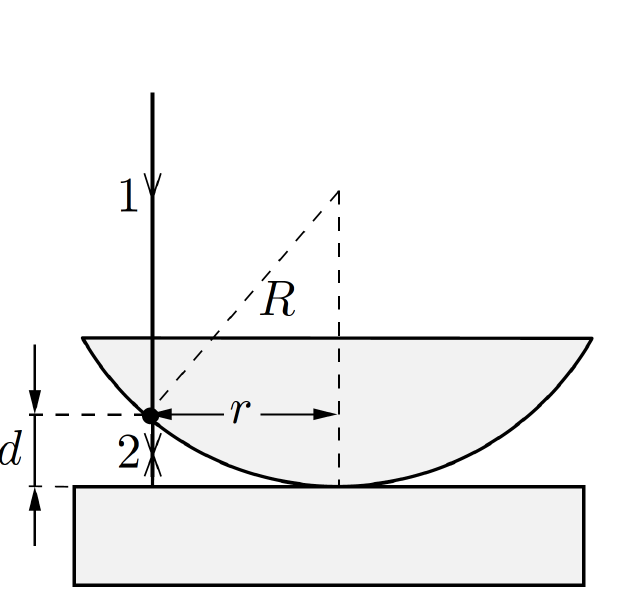
\includegraphics[width=\linewidth]{pics/lens.png}
    \caption{Касающаяся линза}\label{fig:lens}
\end{wrapfigure}

Этот классический опыт используется для определения радиуса кривизны сферических
поверхностей линз. В этом опыте наблюдается интерференция волн, отражённых от границ
тонкой воздушной прослойки, образованной сферической поверхностью линзы и плоской
стеклянной пластиной. При нормальном падении света (рис.~\ref{fig:lens})
интерференционные полосы локализованы на сферической поверхности и являются
полосами равной толщины.
	
Геометрическая разность хода между интерферирующими лучами равна удвоенной толщине
воздушного зазора $ 2d $ в данном месте. Для точки на сферической поверхности,
находящейся на расстоянии $ r $ от оси системы, имеем
$ r^2 = R^2 - {(R - d)}^2 = 2Rd - d^2 $, где $ R $ --- радиус кривизны сферической
поверхности (рис.~\ref{fig:lens}).
	
	При $R\gg d$ получим $d = r^2/2R$. С учётом изменения фазы на $\pi$ при отражении волны от оптически более плотной среды (на границе воздух-стекло) получим \textbf{оптическую разность хода интерферирующих лучей}:
	
\begin{equation}\label{r_m}
    \Delta = \dfrac{\lambda}{2} + 2d = \dfrac{r^2}{R} + \dfrac{\lambda}{2}
\end{equation}
	
Из условия интерференционного минимума
$ \Delta = \dfrac{(2m +1)\lambda}{2}, \; m =0, 1, 2.. $ получим радиусы темных
колец $ r_m $, а из аналогичного условия максимума $ \Delta = m \lambda $
радиусы светлых $r_m'$:
	
\begin{equation}\label{r_m'}
    r_m = \sqrt{m \lambda R}, \qquad r_m' = \sqrt{\dfrac{(2m-1) \lambda R}{2}}
\end{equation}

\section*{Установка}
Схема экспериментальной установки приведена на рис. \ref{ust}. Опыт выполняется с помощью измерительного микроскопа. На столике микроскопа помещается держатель с пластинкой чёрного стекла. На пластинке лежит исследуемая линза.
Источником света служит ртутная лампа, находящаяся в защитном кожухе. Для получения монохроматического света применяется призменный монохроматор, состоящий из конденсора $K$, коллиматора (щель $S$ и объективаа $O$) и призмы прямого зрения $\Pi$. Эти устройства с помощью рейтеров располагаются на оптической скамье. Свет от монохроматора попадает на опак-иллюминатор (ОИ), расположенный между окуляром и объективом микроскопа -- специальное устройство для освещения объекта при работе в отражённом свете. Внутри опак-иллюминатора находится полупрозрачная пластинка $P$, наклонённая под углом 45$^\circ$ к оптической оси микроскопа. Свет частично отражается от этой пластинки, проходит через объектив микроскопа и попадает на исследуемый объект. Пластинка может поворачиваться вокруг горизонтальной оси $x$, а опак-иллюминатор -- вокруг вертикальной оси.
\begin{figure}[H]
    \centering
    
\includegraphics[scale=0.14]{pics/ustanovka.png}
    \caption{Схема установки для наблюдения колец Ньютона}
    \label{ust}
\end{figure}
Столик микроскопа может перемещаться в двух взаимно перпендикулярных направлениях с помощью винтов препаратоводителя. Отсчетный крест окулярной шкалы перемещается перпендикулярно оптической оси микроскопа с помощью микрометрического винта.
Оптическая схема монохроматора позволяет получить в плоскости входного окна опак-иллюминатора достаточно хорошо разделённые линии спектра ртутной лампы. Изображение щели $S$ фокусируется на поверхность линзы объективом микроскопа, и в том же месте находится плоскость наблюдения микроскопа, т.е. точка источника и точка наблюдения интерференции совпадают. Картина интерференции, как и в случае расположения пластинки сверху, так и в данном случае не зависит от коэффициента преломления линзы и определяется величиной зазора между нижней поверхностью линзы и стеклянной пластинкой.
Рекомендуется сначала настроить микроскоп на кольца Ньютона в белом свете (свете ртутной лампы), а затем после выделения монохроматором зелёной линии провести измерения в монохроматическом свете.

\section*{Задание}
\subsection*{Измерения}
\begin{minipage}[]{0.6\textwidth} 
    \textbf{1 - 2.} Настраиваем установку для получения четкого изображения колец и переносим перекрестие в середину центрального пятна.

    \textbf{3.} Определяем координаты диаметров тёмных и светлых колец и оцениваем диаметр пятна соприкосновения линзы со стеклянной пластинкой. Таблица с данными справа.

    \textbf{4. + 7.} При освещении системы светом, содержащим две спектральные компоненты, наблюдается характерная картина биений: чёткость интерферен ционных колец периодически изменяется. Это объясняется наложением двух систем интерференционных колец, возникающих для разных длин волн $\lambda_1$ и $\lambda_2$. Чёткие кольца в результирующей картине образуются при наложении светлых колец на светлые и тёмных на тёмные. Размытые кольца получаются при наложении светлых колец одной картины на тёмные кольца другой. Нетрудно рассчитать период возникающих биений. Пусть в промежутке между двумя центрами соседних чётких участков укладывается $\Delta m$ колец для спектральной линии с длиной волны $\lambda_1$. Тогда в этом промежутке должно располагаться $(\Delta m + 1)$ колец для спектральной линии с длиной волны $\lambda_2$ (при $\lambda_2$ < $\lambda_1$).
Получаем следующее соотношение:
\begin{equation}
    \Delta \lambda = \lambda / \Delta m
    \label{m}
\end{equation}
В процессе выполнения работы было получено $\Delta m = (13 \pm 1)$. Из этого, при $\lambda \approx 540$ нм, следует, что $\Delta \lambda = (38,6 \pm 2,9 )$ нм. Табличное же значение составляет $\Delta \lambda_{\text{табл}} = 33$ нм (значение взято из Лабораторного практикума по физике, Том 2, оптика).
\end{minipage}%
\hfill 
\begin{minipage}[t]{0.35\textwidth} 
    \begin{tabular}{|c|c|}
    \hline
     $r_{\text{темные}}$, мкм   &  $r_{\text{светлые}}$, мкм   \\ \hline
    38 - пятно & 51  \\ \hline
    85  & 101 \\ \hline
    130 & 145 \\ \hline
    159 & 171 \\ \hline
    188 & 200 \\ \hline
    210 & 223 \\ \hline
    231 & 241 \\ \hline
    251 & 259 \\ \hline
    270 & 279 \\ \hline
    286 & 294 \\ \hline
    303 & 312 \\ \hline
    218 & 225 \\ \hline
    232 & 238 \\ \hline
    244 & 253 \\ \hline
    257 & 264 \\ \hline
    270 & 277 \\ \hline
    283 & 291 \\ \hline
    297 & 303 \\ \hline
    308 & 315 \\ \hline
    319 & 323 \\ \hline
    330 & 336 \\ \hline
    339 & 345 \\ \hline
    349 & 353 \\ \hline
    359 & 364 \\ \hline
    367 & 374 \\ \hline
    380 & 385 \\ \hline
    389 & 395 \\ \hline
    401 & 407 \\ \hline
    \end{tabular}
\end{minipage}
Погрешность считаем так: $\delta(\Delta \lambda) = \lambda \cdot \epsilon_{\Delta m} = \lambda \cdot \frac{\delta(\Delta m)}{\Delta m}$.

\subsection*{Обработка результатов}

\textbf{5. - 6.} Подставляем объектную шкалу вместо линзы получаем что в 8 единицах окулярной шкалы лежит 73 единицы  объектной шкалы $\Rightarrow$ цена деления окулярной шкалы равна $(0.091)\pm0.004$ мм/дел. За погрешность берем 3 единицы объектной шкалы: 1 ед за неточность определения границы, 1 ед за наклон, 1 единица за неточность самой шкалы.
\newpage
\textbf{8.} Строим графики по данным из таблицы выше: 
\begin{figure}[h]
\centering
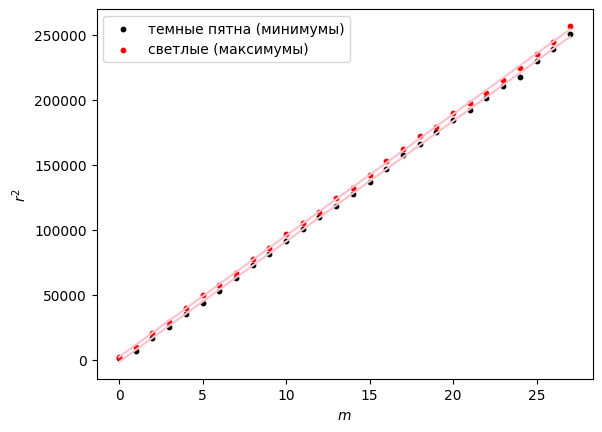
\includegraphics[width=0.45\linewidth]{pics/все.png}
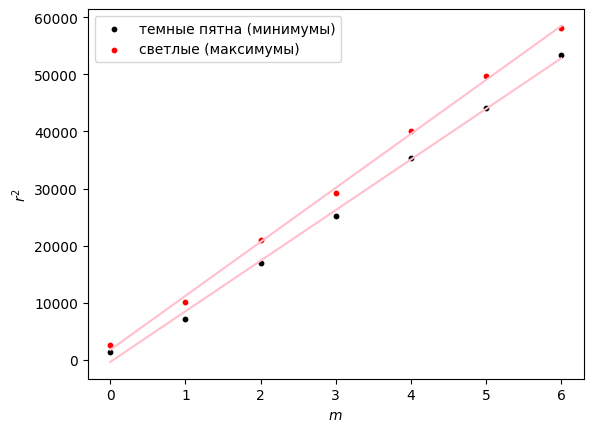
\includegraphics[width=0.45\linewidth]{pics/первые_7.png}
\end{figure}\\
Оценки справедливости линеаризации: 
\begin{equation}
\left\{
\begin{aligned}
    k_d = (9263\pm65), \text{мкм}^2\\
    \frac{\delta k_d}{k_d} = 0.3 \%
\end{aligned}
\right.
\end{equation}
\begin{equation}
\left\{
\begin{aligned}
    k_l = (9335\pm73), \text{мкм}^2\\
    \frac{\delta k_d}{k_d} = 0.4 \%
\end{aligned}
\right.
\end{equation}
Исходя из полученных значений, оценим радиус кривизны линзы:\\
$R_d = (14,60 \pm 0,35)$ $\text{мм}$, $R_l = (15,32
\pm0,41)$ $\text{мм}$\\
Погрешность оцениваем как $\sqrt{\sigma_{\text{случ}}^2 + \sigma_{\text{сист}}^2}$, где $\sigma_{\text{случ}}$ - обычная погрешность из МНК, $\sigma_{\text{сист}} = 2 \frac{\epsilon_r}{\sqrt{N}}$, в качестве систематической ошибки берем ошибку из-за люфта микрометрического винта - 3 мкм, как просто наибольшую из всех остальных.
\section*{Выводы}



\end{document}